\chapter{The File System}
\label{chap-three}
\begin{figure}[hbtp]
\centering
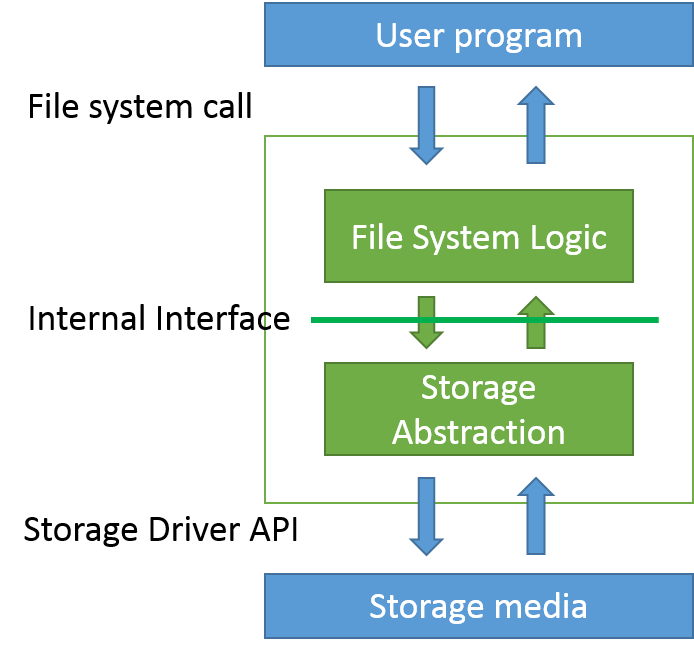
\includegraphics[width=0.5\textwidth]{Chapter-3/figs/fig8.png}
\caption{Modules of Kabi File System}
\label{fig:modules}
\end{figure}

    The file system we implemented (referred as “the Kabi File System” hereafter) can be divided into two internal modules, the storage abstraction module and the file system logic module, as shown in \fref{fig:modules}. The file system logic module decomposes any file system call to series of standard operations to the basic elements in the file system. While the storage abstraction module abstracts the underlying storage media and expose a set of method to the file system logic. There is an internal interface in between that defines several standard method to operate the basic elements. 

    The user program talks to the file system logic through file system APIs. Therefore for different file system API (e.g. FUSE, Dokan, POSIX), we will have different implementation of file system module. The storage abstraction module operates the underlying storage media through its driver, protocol or API. So an implementation of the storage media module is associate with certain storage media (e.g. MongoDB, Volume manager, Amazon S3 service). By using this design, we can easily migrate the file system to other operating system (by changing the file system logic module) or other underlying storage media (by replacing the storage abstraction module).

\begin{figure}[hbtp]
\centering
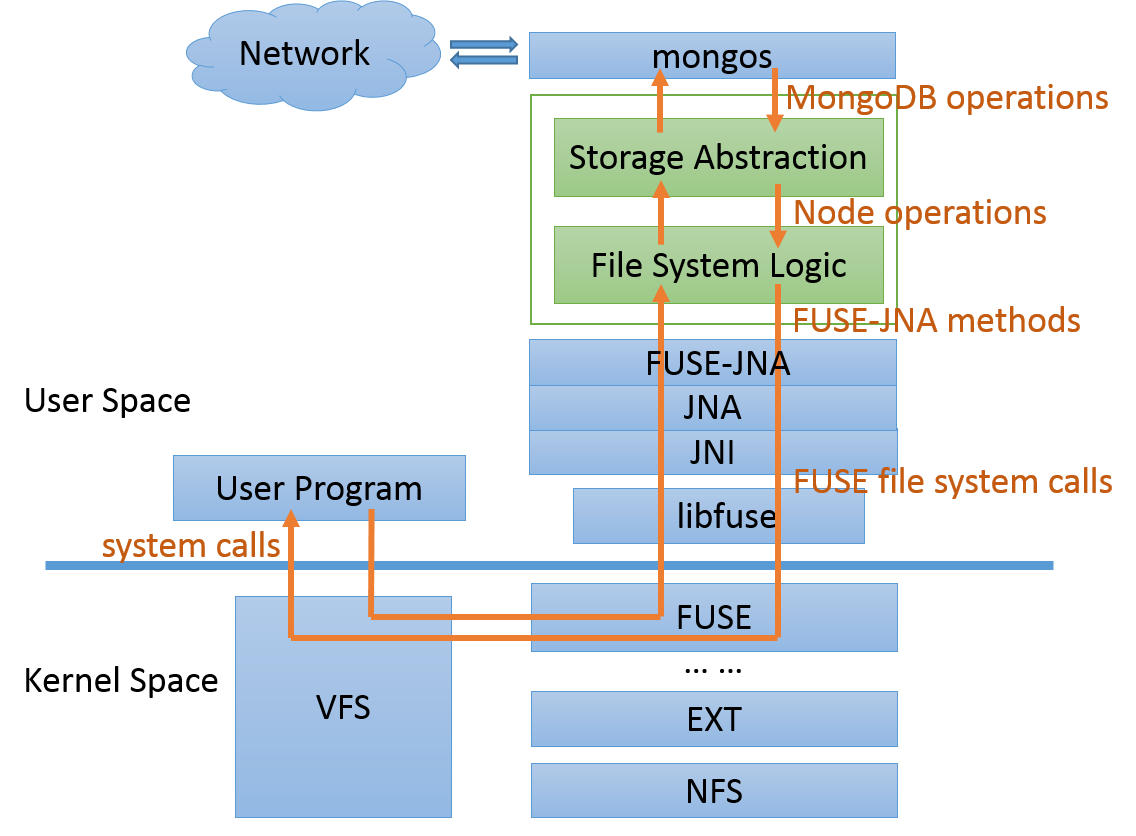
\includegraphics[width=0.8\textwidth]{Chapter-3/figs/fig1.png}
\caption{System Diagram of Kabi File System}
\label{fig:diagram}
\end{figure}

	In our proof-of-concept implementation, FUSE is used to connect the user program file system calls to the Kabi File System. A file system call from a user program will first be captured by VFS module in the kernel and routed to FUSE. FUSE will then pass on the file system call to the file system and pop the return value back to VFS module.

    In order to connect the FUSE dynamic library “libfuse”, an open source project FUSE-JNA is used to map libfuse function to Java methods. The project is slightly modified so as to keep the logging module consistent with the file system. JNA of version 3.5.2 is required by FUSE-JNA to avoid the timestamp issue.

    On the other side, the MongoDB Java driver is used by system abstraction module to communicate with the MongoDB daemon process (Mongos or Mongod).
The system diagram in \fref{fig:diagram} shows the relationship between the file system, MongoDB and operating system.

    On file system initialization, an integer parameter specifying the block size in bytes must be provided. Some optional parameter include the name of the MongoDB collection used by the file system. These parameters provided on initialization will be stored in a special MongoDB collection.

    The file system also requires a JSON format ASCII configuration file on mount. The configuration file should have three sections, specifying the FUSE options, MongoDB options and file system client options. These parameters are important to specify the data source (such as the ip address and server status of MongoDB server), the snapshot to be mounted and the name of the MongoDB collection where the initialization parameter is written.
    
\begin{figure}[hbtp]
\centering
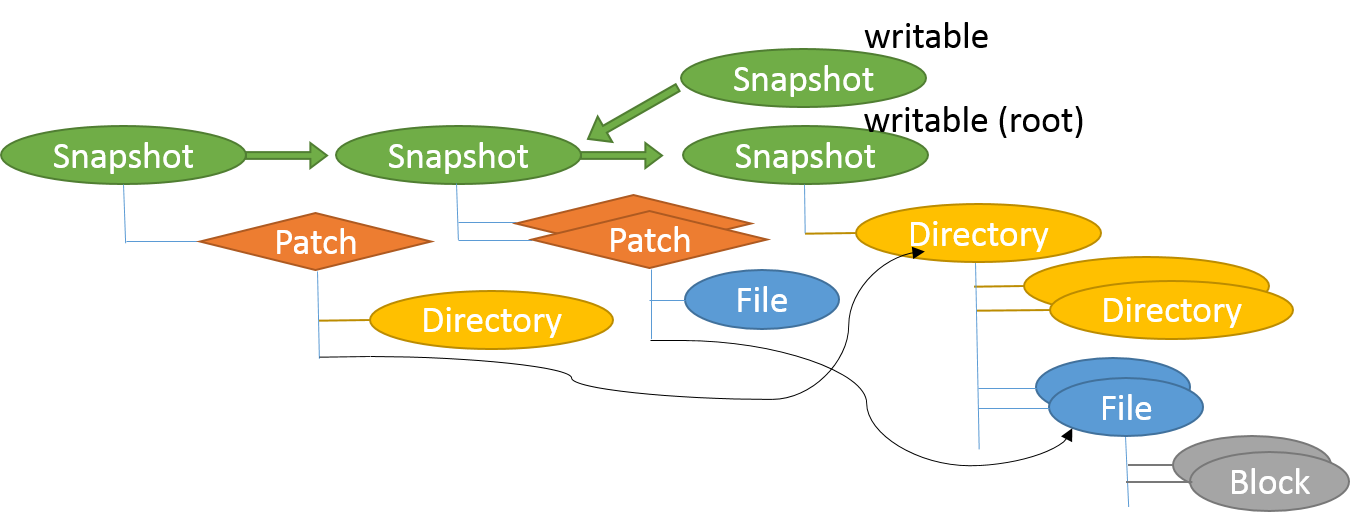
\includegraphics[width=0.9\textwidth]{Chapter-3/figs/fig2.png}
\caption{Basic Entities and Relations}
\label{fig:basic_entities}
\end{figure}

    \fref{fig:basic_entities} shows a basic view of the Kabi File System. The Kabi File System consists of 5 basic type of elements called node: the snapshot node, the patch node, the directory node, the file node and the block node. Nodes are referring to each other and forms a directed acyclic graph. In this implementation, each type of node is stored as a document in a MongoDB collection except for the patch node which is stored as a member object of a snapshot node. 

\section{Nodes}
    Nodes the basic entities defined by the internal interface. They are the inter-media objects between file system logic module and the storage abstraction module. The storage abstraction module manages how these nodes are stored in the MongoDB.
Block nodes are the very basic element in this file system. The block node is a representation of fixed-size binary data. Within a particular instance of the file system, the length of the byte string is immutable, while one can set different value for different instance of the file system on file system initialization. Though the size of data represented by the node is fixed, the node does not have to store that much bytes because the file system will add \'\textbackslash0\' padding at the end when necessary. In addition to the data field, a block node has two other field: a 128 bit hash of the byte string and a 32 bit rolling hash of the byte string. The structure of a typical block node is shown in \ref{tab:block_fields}.

\begin{table}
\caption{Fields in Block Node Object}
\label{tab:block_fields}
\begin{center}
\begin{tabular}{ll}
\toprule
field & remark\\
\midrule
id & the 128 bit SHA hash of bloack data\\
data & the block data\\
\bottomrule
\end{tabular}
\end{center}
\end{table}

    A file nodes is a representation of a certain file in the file system. In the Kabi File System, the content of the file is made up of several sections of variable length and each section is represented through a “data section” bson object. A file node consists a list of data sections and some other meta fields. Connecting the content of data section in order forms the content of the file. Each data section is correspond to exactly one block node and the block node may contribute only part of its binary data to the data section instead of its entire binary data. If only part of block node data is used by the data section, two integers will be specified to locate the start index and end index. \fref{fig:file_and_section} shows a file node consists of 3 data sections where the first data section contributes all 4 byte of corresponding block node data, the second section gets 2 bytes from its corresponding block node and the last section receives the first 2 bytes from its corresponding block node.

\begin{figure}[hbtp]
\centering
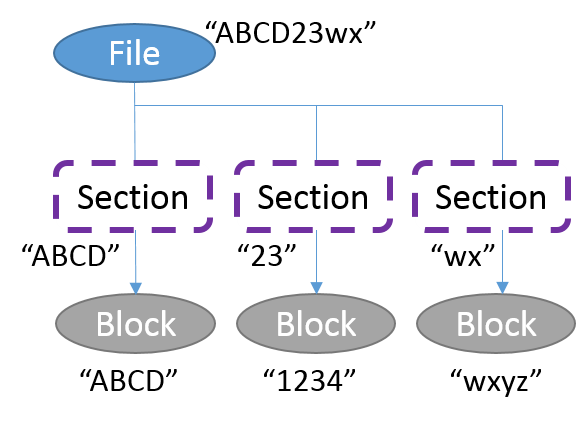
\includegraphics[width=0.5\textwidth]{Chapter-3/figs/fig7.png}
\caption{File Node, Section Object and Block Node}
\label{fig:file_and_section}
\end{figure}

	The detailed structure of a file node is shown in \ref{tab:file_fields}.

\begin{table}
\caption{Fields in File Node Object}
\label{tab:file_fields}
\begin{center}
\begin{tabular}{ll}
\toprule
field & remark\\
\midrule
mode & access mode of the directory\\
arc & a list of Section object\\
size & size of the file\\
owner & owner of the directory\\
gowner & group owner of the directory\\
modified & timestamp for last modification\\
\bottomrule
\end{tabular}
\end{center}
\end{table}

    The data section object is a Mongo bson object. It consists of three basic type as shown in \ref{tab:section_fields}, an object id referring to the associate block node, an integer value specifies the number of omitted leading bytes, another integer value specifies the index of last byte in block node. For the example shown in \fref{fig:section_and_block}, for the second block, the number of omitted leading bytes is 1, and the index of the last byte in block is 5.

\begin{figure}[hbtp]
\centering
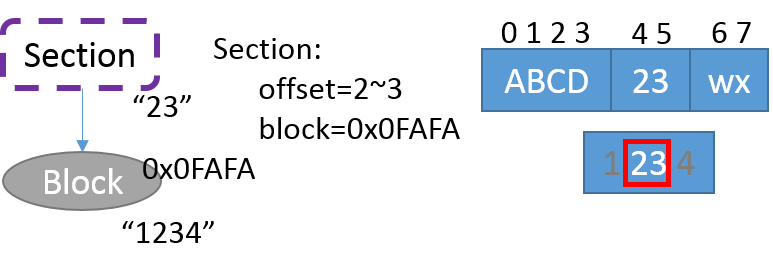
\includegraphics[width=0.9\textwidth]{Chapter-3/figs/fig9.png}
\caption{Section Object and Block Node}
\label{fig:section_and_block}
\end{figure}

\begin{table}
\caption{Fields in Section Object}
\label{tab:section_fields}
\begin{center}
\begin{tabular}{ll}
\toprule
field & remark\\
\midrule
id & id of corresponding \b{block}\\
roll & the 32 bit rolling hash of \b{block} data\\
omit & specify how many leading bytes in block will be omitted\\
offset & the offset of last byte in this \b{section}\\
\bottomrule
\end{tabular}
\end{center}
\end{table}

    Another important field of a file node is the “size”. It stores an integer value, representing the size of this file in bytes. When reading the file, \'\textbackslash0\' padding will be append to the end of files if the “size” value exceeds the total number of bytes in its data sections. On the contrary, if the total number of bytes in data sections exceeds the “size” vale, data will be truncated. This design allows faster creation and truncate operation to a file.

    A directory is represented by a directory node. The structure of a directory is similar to file node. It also consists of fields that store the meta information and a list of subnode object. Similar to the data section object in file node, subnode object is also stored as MongoDB BSON object. It may represent a sub directory or a subfile depending on the type of its referencing node. A subnode object contains a reference to a directory node or a file node, and a string field represents the display name of this subdirectory or subfile.

\begin{table}
\caption{Fields in Directory Node Object}
\label{tab:dir_fields}
\begin{center}
\begin{tabular}{ll}
\toprule
field & remark\\
\midrule
mode & access mode of the directory\\
arc & a list of SubNode object\\
owner & owner of the directory\\
gowner & group owner of the directory\\
modified & timestamp for last modification\\
\bottomrule
\end{tabular}
\end{center}
\end{table}

\begin{table}
\caption{Fields in SubNode Object}
\label{tab:subnode_fields}
\begin{center}
\begin{tabular}{ll}
\toprule
field & remark\\
\midrule
name & display name of the file or subdirectory\\
id & id of the file or subdirectory\\
\bottomrule
\end{tabular}
\end{center}
\end{table}


    The other two types of nodes are patch nodes and snapshot nodes, these two nodes are  related to the snapshot system and will be discussed in the related chapter.

\section{File System Operations}
    The file system logic module decomposes the FUSE file system calls to standard node operations defined by the internal interface. Most of the FUSE file system calls have been implemented in the Kabi File System, some of those important calls include getattr(), access(), read(), write(), rmdir(), unlink(), mkdir(), truncate(), flush(), open() and release(). Related node operations are addDirNode2db(), addFileNode2db(), addDataNode2db() and patch(). The former 3 methods write a node object into the database as a new node. The patch() method replaces an existing node with its new version.

\subsection{Read operations}
    getattr(), access() and read() are three important FUSE function. The access() function tests the existence and permission settings of a file or directory in the file system. getattr() returns the meta information about a file or directory. The read() function reads and return certain length of binary data at a specific offset.
The first step of a read operation is always finding the target file or directory node by path. In order to do so, the file system should parse the given path and find all corresponding nodes on the path in order from root directory to the target. The file system will start with the root directory, keep traversing subnode list and find the directory on the path until the algorithm hit the target or find it nowhere.

    This strategy is generally not satisfactory especially when the target hides deep in the directory tree. In such case, an access call will be mapped to a sequence of database queries on directory nodes and may become a bottleneck in performance. To solve this issue, a cache that stores the path-node relationship is introduced. With the help of the path-node cache, the file system will only query the database when the target directory or file cannot be found in the cache.

    The path-node cache is a move-to-front dictionary which maps the path string to directory node or file node. The cache has a fix capacity and assumes temporal locality in the access pattern. It uses move-to-front algorithm to keep frequently accessed hot item in the cache and remove those cold items that have not been accessed for long. The cache also assumes spatial locality: when accessing a file or directory, not only the file or directory itself is cached but all directories on the path, i.e. its parent and ancestor directories also go into the cache. Thus when visiting contents under the same directory later, the file system will find its parent node in cache.

    Once the file node is retrieved, reading the file is intuitive. The file system will traverse the data section list to find the id of block node associate with the read call and calculate the begin and end index of the bytes of the block content that will be copied to read buffer. After that the file system will query MongoDB for block nodes and copy requested data to buffer.

\subsection{Write operations}

\begin{figure}[hbtp]
\centering
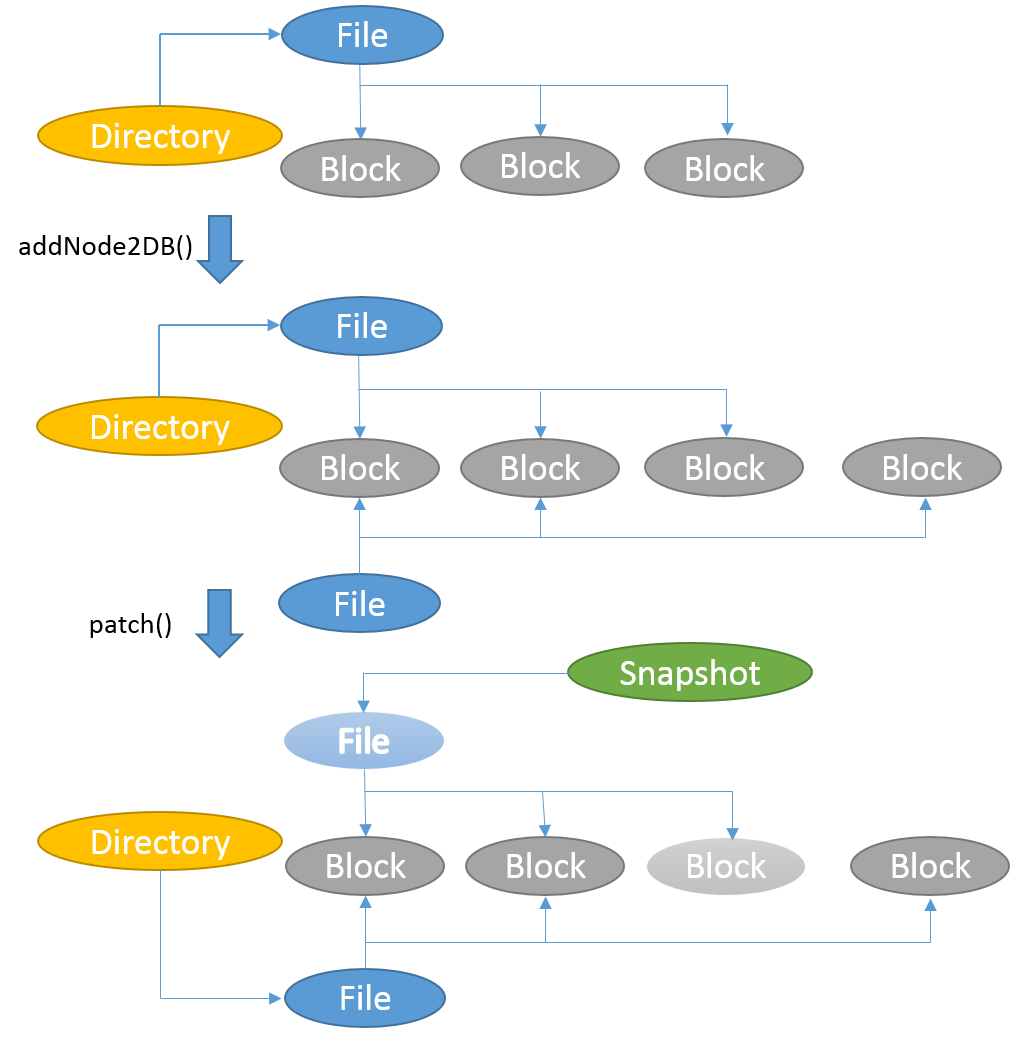
\includegraphics[width=0.8\textwidth]{Chapter-3/figs/fig10.png}
\caption{Copy-on-Write}
\label{fig:cow}
\end{figure}

    Write operations involves FUSE calls named write, chmod, chown, mkdir, unlink and rmdir. The write() call is the most important file system call that writes data into a file from some offset. Other functions change the meta information of a directory or file.

    Block nodes are designed to be immutable, file node and directory nodes uses copy-on-write strategy when an overwrite is requested. So when a overwrite to file node or directory node is requested, the file system will make a local copy of the node and apply the modification to this local copy. The file system will then upload that copy to remote and attach it to its parent directory replacing the pre-modified node as shown in the figure below. In this way, the old version of the node is saved for snapshot and read operation will not accidentally reads in a node in an incomplete state. As shownin \fref{fig:cow}, during this process, we use addNode2DB() operations to add a new node and use the patch() method to replace the old version with this new node.

	When writing a file, the write request will not flush data into persistent storage immediately but instead the data will be written into a local write buffer. Data in write buffer will be merged and subsequent write will overwrite previous buffered data when there is an overlap. When the file system receives a file close request or an explicitly flush request, data in buffer will be truncated into blocks and uploaded to remote servers. \fref{fig:buffer} shows how the buffer works.

\begin{figure}[hbtp]
\centering
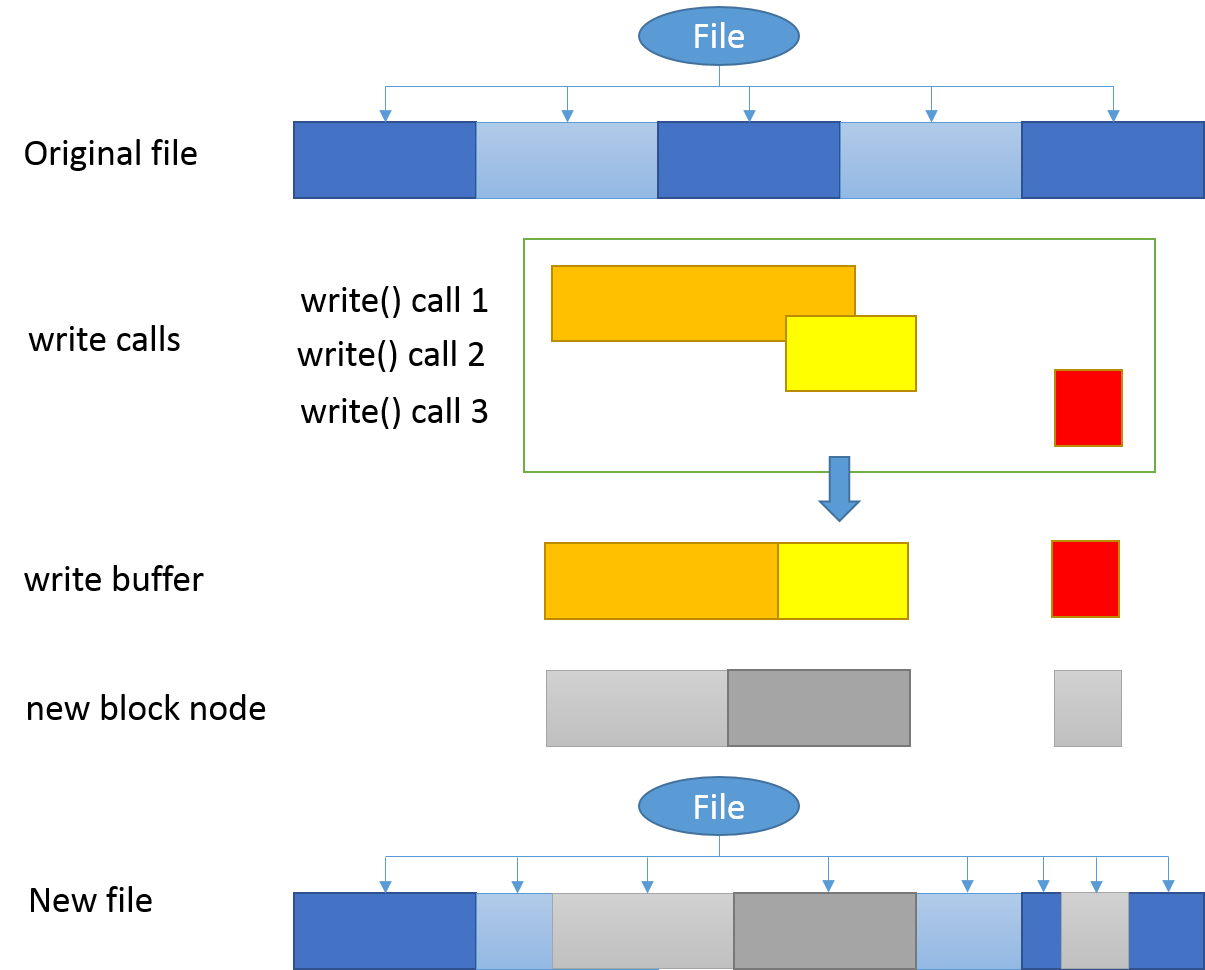
\includegraphics[width=0.8\textwidth]{Chapter-3/figs/fig11.png}
\caption{Write Buffer}
\label{fig:buffer}
\end{figure}

	During a flush, a data section may be unaffected, partly overwritten or entirely overwritten. Block node will be detached from the file if its representing data section has been entirely overwritten. The data section object will be truncated if this section is partly overwritten. The figure below shows the routine to write a file.


    Compared to the traditional copy-on-write snapshot file system which copies and overwrites the entire block whenever there is a byte change, this design can make use of the old block. Since the old block will be referenced by snapshots, reusing it in current view may save some storage for us.
However, there is a trade off between this saving and the overhead of such design. Each data section object requires 224 bit storage to store its SHA hash, rolling hash and begin/end indexes, each block node requires 128 bit to store its SHA id. But the overheads may be worthy. In extreme case, overwriting 2 bytes on the boundary of two block results in two new block to be created in traditional copy-on-write design while only one 2-byte block created in our design. With a block size of 2048 bytes and a file size of 20,480 bytes, this means 3798 bytes in saving.

\subsection{Deduplication}

    In a copy-on-write file system, there is rarely in-place modification to data. In most cases, making a change to the file system means creation of new nodes. On the other hand, creating a new block node is an expensive operation as it requires all data transferred to remote and a permanent reduction of the available space on the storage media.
We found that not all block node creation is necessary. Consider the following scenario, when some user program is trying to create a copy of some certain file to some other location. The program will reads in all data from file to buffer and then write the data in the buffer to another newly created file. As a result, the file system will experience a series of read() and write() function call, without acknowledging that these function calls are related. File system has no way to know that the block node it is going to write already exists in the file system and can be reused.

    By using SHA hash as the block node id, it is possible to find and eliminate blocks that contains duplicate data. Before a block of binary data is uploaded, the file system will query the database with its SHA, if a instance with same id is found, the file system will stop unloading the block node but directly return the id of existing node with same hash value.

    In this way, the file system not only can perform a copy operation efficiently but also find duplicated blocks or similar file and save space when saving them